\newpage
\section{Presentation of the Problem}

The problem that we are trying to solve is the simulation of the propagation of waves. In this section, we present the problem in the context of seismic imaging, an essential component of the seismic processing. We explain its importance in various migration methods, as well as how as a forward problem, numerical simulation is also essential to its counterpart, the inverse problem.

\subsection{Inverse Problem: Seismic Imaging}

Part of the data processing is seismic imaging, whose goal is to produce an accurate image of the underground that geophysicists can interpret to determine the location of hydrocarbon reservoirs. Given the data, a series of pressure or velocity observations by receivers at the surface or at the seafloor, is it possible to reconstruct this image? Since we know the observations as well as one of the inputs (the source signal), and we are looking for the other inputs (the reflection coefficients), seismic imaging is thus an inverse problem whose solution is a collection of parameters we cannot directly observe. As an inverse problem in a physical setting, it is also an ill-posed problem, where we do not have enough information to get a unique solution. However, we may add new pieces of information such as well log data to the system in order to generate a more accurate image. 


One of the methods to solve the inverse problem and create the seismic image is to use Wavefield Extrapolation Migrations, a technique that uses the full wavefield as opposed to ray theory \cite{EAGE}. This class of migration methods includes the recently popular method called Reverse Time Migration or RTM for short, and can be very computationally expensive, requiring up to hundreds or even thousands of cores. The essence of the calculations here lies in the calculation of the reflection coefficient at every point using the back-propagated upgoing wavefield $P_{up}(x,y,z,t)$ (from the receiver) as well as downgoing wavefield $P_{d}(x,y,z,t)$. Under ideal circumstances, the reflection coefficient $r$ is equal to $\frac{P_{up}(x,y,z,t)}{P_d(x,y,z,t)}$ for all time steps $t$. However, circumstances are never ideal and it is a better idea to use the correlation coefficient calculation:

$$r = \frac{\sum\limits_t P_{up}(x,y,z,t) P_d(x,y,z,t)}{\sum\limits_t P_d^2(x,y,z,t) + \epsilon}$$ 

where $\epsilon$ is a small constant to prevent possible division by $0$, and we use summation instead of integration over time because we are using a computer and numerical algorithm.



\subsection{Forward Problem: Simulation of Wave Propagation}

An important part of solving this inverse problem is computing the solution to the forward problem. Since we need to know the values of the upgoing and downgoing wavefield at each time step (the pressure or velocity measurements at every point in the simulated earth), In essence, solving the forward problem, also known as solving the wave equations (or Maxwell's equations in the context of electromagnetism), is the simpler job of numerical simulation of the propagation of waves - the essence of this paper. 


\subsection{Acoustic Wave Equation}

The reason it is also known as solving the wave equation is that we frequently work with domains that are overly complex than the simple one-dimensional uniform case in university Differential Equations courses. The wave equation is simply a partial differential equation that describes the pressure in the domain. In this paper, we work with the simplest wave equation - the acoustic wave equation - and solve it in the time domain as a demonstration of concept:

$$\nabla u(x,t) - \frac{1}{c(x)^2} \frac{\partial^2 u(x,t)}{\partial t^2} = f(x,t)$$

where $u(x,t)$ is the pressure, dependent on space and time, $c(x)$ is the wave propagation velocity, dependent on space, and $f(x,t)$ is the source signal.


For a complex domain with regions of different physical characteristics, it becomes necessary to simulate the solutions numerically in order to visualize the changes in pressure. We give here examples of the solutions that the Hou10ni and Elasticus programs at Inria Magique3D produce, in the frequency and time domain in Figures \ref{fig:Water-Frequency},\ref{fig:Water-Time}: 

\begin{figure}[ht]
	\centering
	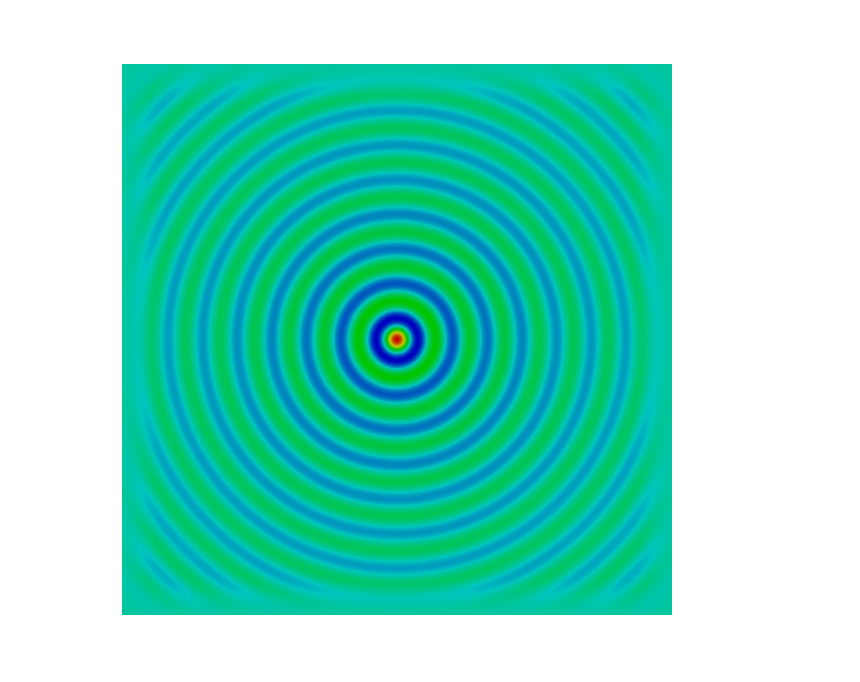
\includegraphics[width=0.7\textwidth]{Images/Water-Frequency.png}
	\caption{Solution to Acoustic Wave Equation in Frequency Domain by Hou10ni program}
	\label{fig:Water-Frequency}
\end{figure}


\begin{figure}
	\centering
	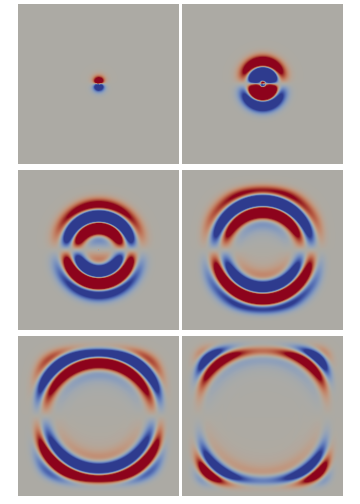
\includegraphics[width=0.9\textwidth]{Images/time.png}
	\caption{Solution to Elastic Wave Equation in Time Domain by Elasticus program}
	\label{fig:Water-Time}
\end{figure}


\subsection{Infinite Domains: Perfectly Matched Layers}

It is also necessary for computational purposes, to limit the size of the computational domain. Although in physical reality, the domain is infinite as the wavefield generated by the source propagates outward, it is necessary to introduce a limit. These limits are currently classified into two major types - Absorbing Boundary Conditions (ABC's) and Perfectly Matched Layers (PML's). Absorbing Boundary Conditions, while more stable in more circumstances than Perfectly Matched Layers, are frequently less effective in mitigating waves incident upon the boundary. For this paper, we use PML, which are easier to implement.

\subsection{Numerical Methods: Discontinuous Galerkin}

There are many numerical methods being used to solve differential equations today, frequently in the domain of structural analysis, including Finite Difference Method (FDM), Finite Element Method (FEM), Finite Volume Method (FVM), and finally Discontinuous Galerkin Methods (DG). The core of these methods lies at the calculation of the desired variable at many points in the domain, frequently using a mesh, whether structured or unstructured, to do so. There exist methods to calculate variables at fluidly changing coordinates without the use of a mesh, notably Smoothed Particle Hydrodynamics, but currently most applications do not use these methods. 

While today, the most popular is FEM for its flexibility in creating meshes that fit well to arbitrary domains, we use the method of Discontinuous Galerkin for this paper.




%\subsubsection{Anisotropy}

%\subsubsection{Elasticity Tensor C}

